\documentclass[A4,12PT, english, twocolumn]{journal}
\usepackage{amsmath,amssymb,amsfonts}
\usepackage[margin=0.7in]{geometry}
\usepackage{graphicx}
\usepackage{enumitem}
\usepackage{xcolor}
\usepackage{hyperref}
\usepackage{tabularray}
\usepackage{multicol}
\usepackage{tikz}
\usepackage{circuitikz}
\usepackage{scalerel}
\usepackage{pict2e}
\usepackage{tkz-euclide}
\usetikzlibrary{calc}
\usetikzlibrary{patterns,arrows.meta}
\usetikzlibrary{shadows}
\usetikzlibrary{external}

%pgfplots
\usepackage{pgfplots}
\pgfplotsset{compat=newest}
\usepgfplotslibrary{statistics}
\usepgfplotslibrary{fillbetween}

\def\infinity{\rotatebox{90}{8}}

% Hiperlink
\hypersetup{
    colorlinks=true,
    linkcolor=blue,
    filecolor=magenta,      
    urlcolor=cyan,
    pdftitle={Overleaf Example},
    pdfpagemode=FullScreen,
}
%\usepackage{style}
\NewDocumentCommand{\Log}{o}{%
\IfNoValueTF{#1}{}{{}^{#1}\!}\log}%
  
%command buat logaritma dengan basisnya di pojok kiri
%\textheight=17cm
%\textwidth=10cm
%\usepackage{blindtext}
\setenumerate[1]{itemsep=0,5cm}
\setenumerate[2]{topsep=5pt, itemsep=5pt, label=\textbf{\Alph*}.}

\title{Matematika Saintek \& Fisika UTUL UGM 2014 Kode 531}
\author{Fauzan Akbar Sukandar Putra \\ \LaTeX}

\begin{document}

\maketitle

%\begin{minipage}{0.5\textwidth}
\begin{enumerate}

%1%
\item Jika garis $y=mx+k$ menyinggung lingkaran \\ $x^2+y^2-10x+6y+24=0$ di titik $(8,-4)$, maka nilai $m+k$ adalah\dots
    \begin{enumerate}
        \item $-26$
        \item $-25$
        \item $-24$
        \item $-23$
        \item $-22$
    \end{enumerate}

%2%
\item Diberikan segitiga $ABC$ dengan $\angle A=\alpha$, $\angle B=90^\circ$, dan $\angle C=\gamma$. Jika $\cos{\alpha}=x$, maka $\cos{\left(\alpha+2\gamma \right)}=$\dots
    \begin{enumerate}
        \item $-x$
        \item $-\sqrt{1-x^2}$
        \item $x$
        \item $\sqrt{1-x^2}$
        \item $1$
    \end{enumerate}

%3%
\item Diketahui matriks $A$ berukuran $3\times 3$ dan memenuhi
\begin{center}
    $
    A\begin{pmatrix}
        1\\
        2\\
        3\\
    \end{pmatrix}=
    \begin{pmatrix}
        2\\
        2\\
        2\\
    \end{pmatrix}
    $ dan
    $
    A\begin{pmatrix}
        1\\
        2\\
        3\\
    \end{pmatrix}=
    \begin{pmatrix}
        2\\
        4\\
        2\\
    \end{pmatrix}
    $.
\end{center}
jika $x=\begin{pmatrix}
            2\\
            4\\
            10\\
        \end{pmatrix}$ maka $Ax=$\dots
    \begin{enumerate}
        \item $\begin{pmatrix}
                    8\\
                    4\\
                    8\\
                \end{pmatrix}$
        \item $\begin{pmatrix}
                    4\\
                    12\\
                    4\\
                \end{pmatrix}$
        \item $\begin{pmatrix}
                    12\\
                    8\\
                    12\\
                \end{pmatrix}$
        \item $\begin{pmatrix}
                    4\\
                    8\\
                    4\\
                \end{pmatrix}$
        \item $\begin{pmatrix}
                    8\\
                    12\\
                    8\\
                \end{pmatrix}$
    \end{enumerate}

%4%
\item Diketahui vektor $\Vec{a}$ dan $\Vec{b}$ membentuk sudut sebesar $\theta$. Jika panjang proyeksi vektor $\Vec{b}$ pada $\Vec{a}$ sama dengan $2\sin{\theta}$ dan panjang $\Vec{b}$ adalah $1$, maka $\tan{2\theta}=$\dots
    \begin{enumerate}
        \item $\frac{1}{3}$
        \item $\frac{2}{3}$
        \item $1$
        \item $\frac{4}{3}$
        \item $\frac{5}{3}$
    \end{enumerate}

%5%
\item Sebuah prisma $ABCD.EFGH$ memiliki alas berbentuk persegi. Titik $T$ adalah titik tengah diagonal $HF$. Jika $\angle EAT=\frac{\pi}{6}$ dan volume prisma tersebut $4\sqrt{6}$, maka tinggi prisma adalah\dots
    \begin{enumerate}
        \item $\sqrt{6}$
        \item $\sqrt{3}$
        \item $\sqrt{2}$
        \item $\frac{\sqrt{3}}{2}$
        \item $\frac{\sqrt{2}}{2}$
    \end{enumerate}

%6%
\item Semua nilai $a$ agar
\begin{center}
    $\sqrt{2x^2-x+14} \geq \sqrt{x^2-ax+10}$
\end{center}
benar untuk semua bilangan real $x$ adalah\dots
    \begin{enumerate}
        \item $\left|a \right| \leq 6$
        \item $a \leq -3$ atau $a \geq 5$
        \item $a \leq -5$ atau $a \geq 3$
        \item $-3 \leq a \leq 5$
        \item $-6 \leq a \leq -5$ atau $3 \leq a \leq 6$
    \end{enumerate}

%7%
\item Jika $P(x)=x^5+ax^4+x^2+bx+2$ dibagi \\ $h(x)=x^3+2x^2-x-2$ memberikan sisa \\ $r(x)=x^2-3x+4$ maka $a+b=$\dots
    \begin{enumerate}
        \item $-2$
        \item $-1$
        \item $1$
        \item $2$
        \item $3$
    \end{enumerate}

%8%
\item Jika $a$ memenuhi persamaan
\begin{center}
    $^2\Log{2x}+ \, ^3\Log{3x}= \, ^4\Log{4x^2}$
\end{center}
maka $^a\Log{3}=$\dots
    \begin{enumerate}
        \item $-3$
        \item $-2$
        \item $-1$
        \item $1$
        \item $2$
    \end{enumerate}

%9%
\item Diketahui jumlahan empat suku pertama suatu barisan aritmatika sama dengan jumlahan tiga suku selanjutnya. Jika jumlah $10$ suku pertamanya adalah $270$, maka suku pertama barisan tersebut adalah\dots
    \begin{enumerate}
        \item $2$
        \item $3$
        \item $6$
        \item $9$
        \item $18$
    \end{enumerate}

%10%
\item Diketahui $f(x)=\sqrt{1+x}$. Nilai
\begin{center}
    $\lim\limits_{h \longrightarrow 0} \dfrac{f\left(3+2h^2 \right)-f\left(3-3h^2 \right)}{h^2}$
\end{center}
adalah\dots
    \begin{enumerate}
        \item $0$
        \item $\frac{2}{3}$
        \item $\frac{6}{7}$
        \item $\frac{9}{8}$
        \item $\frac{5}{4}$
    \end{enumerate}

%11%
\item Jika $f(x)=\left(\sin{x}+\cos{x} \right)\left(\cos{2x}+\sin{2x} \right)$ dan $f'(x)=2\cos{3x}+g(x)$, maka $g(x)=$\dots
    \begin{enumerate}
        \item $\cos{3x}+\sin{x}$
        \item $\cos{3x}-\sin{x}$
        \item $\cos{x}+\sin{x}$
        \item $\cos{x}-\sin{x}$
        \item $-\cos{x}+\sin{x}$
    \end{enumerate}

%12%
\item Diketahui $D_1$ adalah daerah di kuadran $1$ yang dibatasi oleh parabola $y=\frac{9}{4}x^2$, parabola $y=x^2$, dan garis $x=2$, dan $D_2$ daerah yang dibatasi oleh garis $x=2$, garis $y=9$, dan parabola $y=x^2$. Jika luas $D_1=a$, maka luas $D_2$ adalah\dots
    \begin{enumerate}
        \item $\frac{7}{10}a$
        \item $\frac{8}{10}a$
        \item $\frac{9}{10}a$
        \item $\frac{11}{10}a$
        \item $\frac{13}{10}a$
    \end{enumerate}

%13%
\item Tiga pria dan empat wanita akan duduk dalam satu baris. Banyak cara mereka duduk sehingga yang berjenis kelamin sama tidak berdampingan adalah\dots
    \begin{enumerate}
        \item $24$
        \item $49$
        \item $144$
        \item $288$
        \item $5040$
    \end{enumerate}

%14%
\item Untuk setiap bilangan asli $n$ didefinisikan matriks \begin{center}
    $A_n=$ 
    $
    \begin{pmatrix}
        n & 2n\\
        3n & 4n\\
    \end{pmatrix}
    $
\end{center}
Jika $det(A_1+A_2+...+A_k)=-4050$, maka $det(A_{2k})=$\dots
    \begin{enumerate}
        \item $-800$
        \item $-648$
        \item $-512$
        \item $-392$
        \item $-288$
    \end{enumerate}

%15%
\item Diketahui persamaan $x^2+px+q=0$ mempunyai akar-akar positif $x_1$ dan $x_2$. Jika $x_1, \; 6, \; x_2$ adalah tiga suku pertama barisan geometri dan $x_1, \; x_2, \; 14$ tiga suku pertama barisan aritmatika, maka $p+q=$\dots
    \begin{enumerate}
        \item $23$
        \item $24$
        \item $25$
        \item $26$
        \item $27$
    \end{enumerate}
    
    
%FISIKA %
%16%
\newpage
\item Lima buah balok di atas lantai licin, disusun dan dikenai gaya $100 \; N$ seperti dilukiskan oleh gambar dibawah. Besar tegangan tali $4$ adalah\dots
\begin{center}
    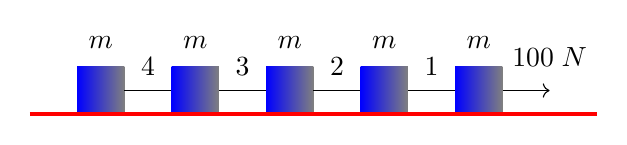
\begin{tikzpicture}[scale=0.6]
    %GRID
    %\draw[lightgray] (0,0) grid (10,5);
    %GAYA
    \draw[black, ->] (1,0.5) to (11,0.5) node[above=5pt] {$100 \; N$};
    %ANOTASI m
    \shade[left color=blue, right color=gray] (1,1) -- (2,1) node[midway, above=3pt] {$m$};
    \shade[left color=blue, right color=gray] (3,1) -- (4,1) node[midway, above=3pt] {$m$};
    \shade[left color=blue, right color=gray] (5,1) -- (6,1) node[midway, above=3pt] {$m$};
    \shade[left color=blue, right color=gray] (7,1) -- (8,1) node[midway, above=3pt] {$m$};
    \shade[left color=blue, right color=gray] (9,1) -- (10,1) node[midway, above=3pt] {$m$};
    %KOTAK-KOTAK
    \shade[left color=blue, right color=gray] (1,0) rectangle (2,1);
        \draw (2,0.5) -- (3,0.5) node[midway, above=2pt] {$4$};  
    \shade[left color=blue, right color=gray] (3,0) rectangle (4,1);
        \draw (4,0.5) -- (5,0.5) node[midway, above=2pt] {$3$};  
    \shade[left color=blue, right color=gray] (5,0) rectangle (6,1);
        \draw (6,0.5) -- (7,0.5) node[midway, above=2pt] {$2$};  
    \shade[left color=blue, right color=gray] (7,0) rectangle (8,1);
        \draw (8,0.5) -- (9,0.5) node[midway, above=2pt] {$1$};  
    \shade[left color=blue, right color=gray] (9,0) rectangle (10,1);
    %LANTAI%
    \draw[ultra thick, red] (0,0) -- (12,0);
    \end{tikzpicture}
\end{center}
    \begin{enumerate}
        \item $20 \; N$
        \item $25 \; N$
        \item $40 \; N$
        \item $50 \; N$
        \item $80 \; N$
    \end{enumerate}
  
%17%
\item Pada $t=0$ kelereng $X$ mulai jatuh bebas dari ketinggian $H$ dan tepat dibawahnya kelereng $Y$ dilempar ke atas dari permukaan tanah dengan kecepatan awal $v_0$. Tumbukan keduanya terjadi pada $t=$\dots
    \begin{enumerate}
        \item $\sqrt{\frac{2h}{g}}$
        \item $\sqrt{\frac{h}{2g}}$
        \item $\frac{2h}{v_0}$
        \item $\frac{h}{2v_0}$
        \item $\frac{h}{v_0}$
    \end{enumerate}
     
%18%
\item Batu dengan massa $10 \; kg$ jatuh mengenai sebuah paku sehingga paku tersebut tembus ke dalam kayu sejauh $0,02 \; m$. Bila kelajuan batu saat mengenai paku adalah $20 \; m/s$, maka besar gaya rata-rata yang diberikan batu pada paku adalah\dots
    \begin{enumerate}
        \item $100.000 \; N$
        \item $10.000 \; N$
        \item $1.000 \; N$
        \item $100 \; N$
        \item $10\; N$
    \end{enumerate}
   
%19% 
\item Sebuah silinder terbuat dari bahan elastik. Penampang silinder memiliki jari-jari $1 \; cm$, sedang panjangnya $20 \; cm$. Tetapan elastik silinder itu $0,8 \; N/m$. Jika bahan itu dilubangi dengan lubang berupa silinder pula yang memanjang sumbu silinder itu dengan jari-jari lubang $0,5 \; cm$, berapakah tetapan elastik silinder dengan lubang itu\dots
    \begin{enumerate}
        \item $0,2 \; N/m$
        \item $0,4 \; N/m$
        \item $0,6 \; N/m$
        \item $0,8 \; N/m$
        \item $1,0 \; N/m$
    \end{enumerate}

%20%
\item Sebuah bandul bermassa $m$ dan panjang tali $L$ mula-mula diam pada posisi tali membentuk sudut \\ $\theta=60^\circ$ terhadap vertikal. Besar gaya tegangan tali saat massa $m$ melewati titik terendah $A$ adalah\dots
\begin{center}
    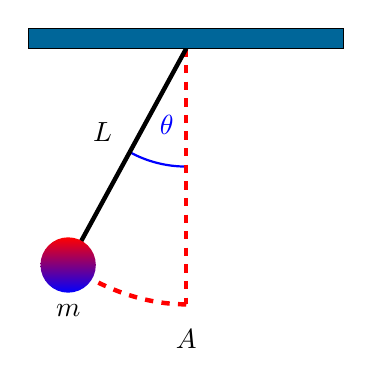
\begin{tikzpicture}
        %GRID
        %\draw[lightgray] (0,0) grid (8,8);
        %SUDUT
        \coordinate (P) at (2,4.75);
        \coordinate (Q) at (0.5,5.25);
        \coordinate (R) at (2,8);
        \draw[ultra thick, dashed, red] (P) parabola (Q);
        \tkzMarkAngle[thick, blue, size=1.5cm](Q,R,P);
        \tkzLabelAngle[blue](Q,R,P){$\theta$}
        %GARIS BANTU 
        \draw[ultra thick, dashed, red] (2,8) -- (2,4.75) node[below=5pt, black] {$A$};
        %GARIS HUBUNG BANDUL
        \draw[ultra thick] (2,8) -- (0.5,5.25) node[below=10pt] {$m$} node[midway, above left=2pt] {$L$};
        %BANDUL
        \shade[top color=red, bottom color=blue] (0.5,5.25) circle (10pt);
        %ATAP
        \filldraw[fill=blue!60!green, draw=black] (0,8) rectangle (4,8.25);
    \end{tikzpicture}
\end{center}
    \begin{enumerate}
        \item $mg$
        \item $2mg$
        \item $\left(3-\frac{1}{2}\sqrt{3} \right)mg$
        \item $\left(3-\frac{1}{2}\sqrt{2} \right)mg$
        \item $3mg$
    \end{enumerate}

%21%
\item Sebuah mobil ambulans yang menyalakan sirine bergerak menuju suatu perempatan lalu lintas. Orang yang diam di perempatan tersebut mendengar frekuensi sirine sebesar $900 \; Hz$ ketika ambulans mendekati perempatan, dan frekuensi sebesar $800 \; Hz$ ketika ambulans tersebut menjauhi perempatan. Asumsikan kecepatan ambulans konstan dan kecepatan bunyi di udara $=340 \; m/s$. Kecepatan ambulans tersebut adalah\dots
    \begin{enumerate}
        \item $72 \; km/jam$
        \item $60 \; km/jam$
        \item $54 \; km/jam$
        \item $48 \; km/jam$
        \item $36 \; km/jam$
    \end{enumerate}
    
%22% 
\item Sumber bunyi mendekati pendengar yang diam dengan kecepatan $v_s$. Ketika sumber memancarkan bunyi dengan frekuensi $400 \; Hz$, pendengar mendengar bunyi tersebut dengan frekuensi $500 \; Hz$. Apabila kecepatan bunyi di udara adalah $v$, nilai $\frac{v_s}{v}$ adalah\dots
    \begin{enumerate}
        \item $\frac{1}{5}$
        \item $\frac{1}{4}$
        \item $\frac{4}{5}$
        \item $\frac{6}{5}$
        \item $\frac{5}{4}$
    \end{enumerate}
    
%23%
\item Seutas kawat penghantar dibentuk seperti pada gambar. Bagian yang melengkung merupakan seperempat lingkaran. Hitung medan magnet di titik $A$ yang merupakan titik pusat lingkaran, tentukan arahnya.
\begin{center}
    \begin{tikzpicture}
        %GRID
        %\draw[lightgray] (0,0) grid (7,7);
        %KOORDINAT
        \coordinate (A) at (2,3);
        \coordinate (B) at (4,3);
        \coordinate (C) at (0,7);
        \coordinate (D) at (0,5);
        \coordinate (E) at (0,3);
        %GARIS & BUSUR
        \draw[ultra thick] (A) -- (B) node [currarrow, pos=0.5, sloped, xscale=1, scale=5, blue] {} arc [start angle=0, end angle=90, x radius=4, y radius=4] node [currarrow, pos=0.5, sloped, xscale=-1, scale=5, blue] {};
        
        \draw[ultra thick] (C) -- (D) node [currarrow, pos=0.5, sloped, xscale=1, scale=5, blue];
        \draw[ultra thick] (A) arc [start angle=0, end angle=90, x radius=2, y radius=2] node [currarrow, pos=0.5, sloped, xscale=1, scale=5, blue];
        
        %CIRCLE
        \filldraw (E) circle (4pt) node [above=20pt, left=3pt] {\Large $A$};
        %GARIS BANTU 
        \draw[ultra thick, blue, dashed, Stealth-Stealth] (0,2.75) -- (2,2.75) node [midway, above=4pt] {\Large $r$};

        \draw[ultra thick, red, dashed, Stealth-Stealth] (0,2.25) -- (4,2.25) node [midway, below=3pt] {\Large $R$}; 
        
    \end{tikzpicture}
\end{center}
    \begin{enumerate}
        \item $\frac{\mu_0 i(R-r)}{8Rr}$, keluar dari bidang gambar
        \item $\frac{\mu_0 i(R-r)}{8Rr}$, masuk ke dalam bidang gambar
        \item $\frac{\mu_0 i}{8(R-r)}$, keluar bidang gambar
        \item $\frac{\mu_0 i}{8(R-r)}$, masuk ke dalam bidang gambar
        \item nol
    \end{enumerate}
    
%24%  
\item Sebuah partikel bermassa $m$ dan bermuatan $q$ mula-mula berada di titik $A$ diatas permukaan meja. Pada ruang di atas permukaan meja itu terdapat medan magnet seragam berarah vertikal ke bawah. Pada saat $t_0$ partikel diberi kecepatan awal dengan komponen vertikal $u_0$ dan mendatar $v_0$. Akibatnya partikel akan bergerak dengan lintasan berupa spiral vertikal ke atas. Berapakah ketinggian partikel itu diukur dari permukaan meja ketika untuk kedua kalinya partikel itu berada diatas titik $A$?
\begin{center}
    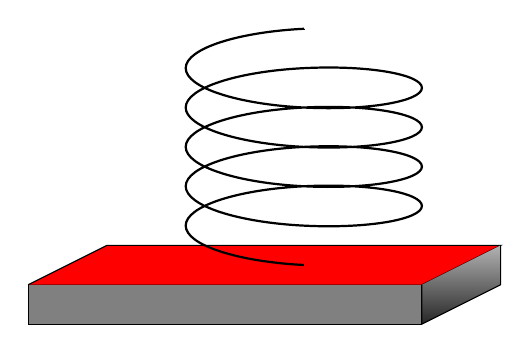
\begin{tikzpicture}
        %GRID
        %\draw[lightgray] (0,0) grid (6,5)[on grid];
        %MEJA 
        
        \filldraw[fill=gray, draw=black] (0,0) rectangle (5,0.5);
        \filldraw[fill=red] (0,0.5) -- (1,1) -- (6,1) -- (5,0.5);
        \shadedraw[top color=white!40!gray, bottom color = black!70!gray] (6,1) -- (6,0.5) -- (5,0) -- (5,0.5);
        %SPRING
        \draw
[      
        thick,
        decoration={
        coil,
        segment length = 5mm,
        amplitude = 15mm,
        aspect = 0.25,
        post length = 0mm,
        pre length = 0mm},
    decorate] (3.5,0.75) -- ++(0,3);        
    \end{tikzpicture}
\end{center}
	\begin{enumerate}
		\item $\frac{m \pi}{qB}(v_0+u_0)$
		\item $4\frac{m \pi}{qB}(u_0+v_0)$
		\item $\frac{2m \pi}{qB}u_0$
		\item $4\frac{m \pi}{qB}u_0$
		\item $4\frac{m \pi}{qB}v_0$
	\end{enumerate}
	
%25%
\item Seutas kawat penghantar dibentuk menjadi bangun seperti pada gambar. Sisi-sisi bangun itu panjangnya $l$. Kawat itu dialiri arus sebesar $i$ dan diletakkan dalam medan magnet $B$ yang berarah masuk bidang gambar tegak lurus. kemana arah gaya total yang dialami oleh bangun itu?
\begin{center}
    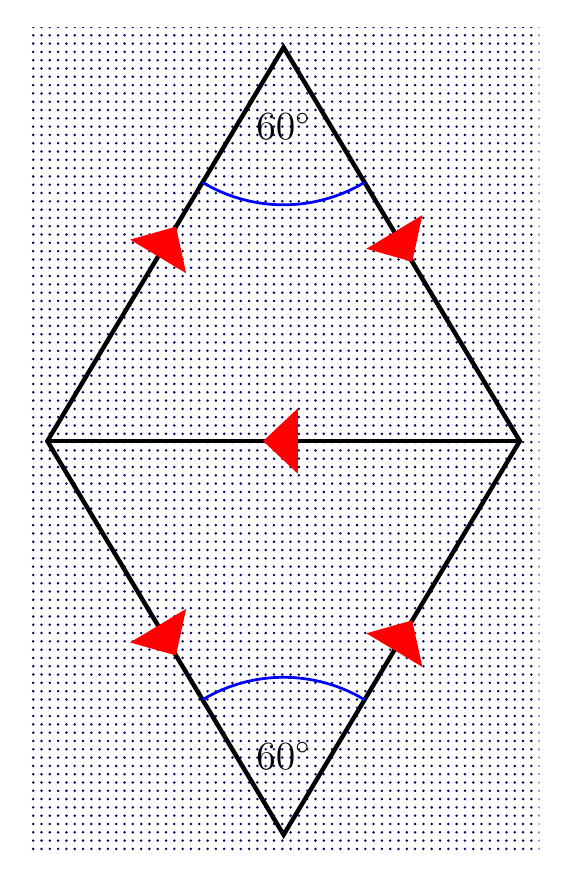
\begin{tikzpicture}
        %GRID
        %\draw[blue] (0,0) grid (6,10);
        %POLA
        \fill[pattern=dots,pattern color=blue!40!black] (-0.25,-0.25) rectangle (6.25,10.25);
        %KOORDINAT
        \coordinate (A) at (3,0);
        \coordinate (B) at (6,5);
        \coordinate (C) at (3,10);
        \coordinate (D) at (0,5);
        %GARIS
        \draw[ultra thick] (A) -- node [currarrow, sloped, scale=5, pos=0.5, xscale=0.5, red] {} (B)  -- node [currarrow, sloped, scale=5, pos=0.5, xscale=0.5, red] {} (C) -- node [currarrow, sloped, scale=5, pos=0.5, xscale=0.5, red] {} (D) -- node [currarrow, sloped, scale=5, pos=0.5, xscale=0.5, red] {} cycle;
        \draw[ultra thick] (B) -- node [currarrow, sloped, scale=5, pos=0.5, xscale=-0.5, red] {} (D);
        %SUDUT
        \tkzMarkAngle[line width=1pt, blue, size=2](B,A,D);
        \tkzLabelAngle (B,A,D) {\Large $60^\circ$};
        
        \tkzMarkAngle[line width=1pt, blue, size=2](D,C,B);
        \tkzLabelAngle (D,C,B) {\Large $60^\circ$};
    \end{tikzpicture}
\end{center}
   \begin{enumerate}
        \item Ke atas
        \item Ke bawah
        \item Ke kiri
        \item Ke kanan
        \item Gaya magnet total nol
   \end{enumerate}
   
%26%
\item Jika model atom Thompson benar, maka sinar alfa yang ditembakkan pada lembaran emas yang tipis akan\dots
    \begin{enumerate}
        \item Diteruskan semuanya dengan pembelokan yang tidak berarti
        \item Dibelokkan sejauh $90^\circ$
        \item Dibelokkan sejauh $130^\circ$
        \item Akan dipantulkan kembali ke sumber
        \item Tidak akan mampu menembus lembaran emas
    \end{enumerate}
  
%27%  
\item Sebuah unsur radioaktif $X$ meluruh, sehingga setelah berturut-turut $6$ hari dan $9$ hari, banyaknya unsur $X$ yang tersisa berturut-turut $40$ gram dan $20$ gram. Banyaknya unsur $X$  mula-mula adalah\dots
    \begin{enumerate}
        \item $640$ gram
        \item $480$ gram
        \item $320$ gram
        \item $160$ gram
        \item $80$ gram
    \end{enumerate}
    
%28%  
\item Sebuah pesawat bergerak dengan kecepatan relativistik sebesar $v$ terhadap bumi. Oleh pengamat di bumi, pesawat itu terukur memiliki panjang $L$. Jika kecepatan pesawat itu diturunkan menjadi setengahnya, panjang pesawat itu terukur oleh pengamat di bumi menjadi $2L$. nilai $v$ sama dengan\dots
    \begin{enumerate}
        \item $\frac{\sqrt{3}}{3}c$
        \item $\frac{2\sqrt{5}}{5}c$
        \item $\frac{c}{2}$
        \item $\frac{\sqrt{6}}{3}c$
        \item $\frac{\sqrt{2}}{2}c$
    \end{enumerate}

%29%  
\item Sebuah partikel mengalami gerak harmonik sederhana dengan amplitudo $5 \; cm$. Saat simpangannya $3 \; cm$, kecepatannya $80\pi \; cm/s$. Frekuensi geraknya adalah\dots
    \begin{enumerate}
        \item $16 \; Hz$
        \item $10 \; Hz$
        \item $8 \; Hz$
        \item $5 \; Hz$
        \item $4 \; Hz$
    \end{enumerate}

%30%
\item Dua buah satelit $A$ dan $B$ mengorbit planet $Z$ masing-masing pada ketinggian $400 \; km$ dan $5400 \; km$ dari permukaan planet tersebut, dengan periode masing-masing berturut-turut $8$ hari dan $27$ hari. Jari-jari planet $Z$ tersebut adalah\dots
    \begin{enumerate}
        \item $1200 \; km$
        \item $2000 \; km$
        \item $2400\; km$
        \item $3000 \; km$
        \item $3600 \; km$
    \end{enumerate}
 
%31%
\item Sebuah planet bermassa $m$ bergerak mengitari matahari bermassa $M$ dalam orbit berbentuk lingkaran berjari-jari $R$. Bila diandaikan matahari rehat (diam), maka besar energi total sistem $E$, adalah\dots
    \begin{enumerate}
        \item $E= \frac{GMm}{r}$
        \item $E= -\frac{GMm}{r}$
        \item $E= -\frac{GMm}{2r}$
        \item $E= \frac{GMm}{2r}$
        \item $E= -\frac{GMm}{2r^2}$
    \end{enumerate}

%32%
\item Benda bersuhu $50^\circ \; C$. Jika diukur dengan termometer Fahrenheit, suhu benda tersebut adalah\dots
    \begin{enumerate}
        \item $162^\circ \; F$
        \item $152^\circ \; F$
        \item $142^\circ \; F$
        \item $132^\circ \; F$
        \item $122^\circ \; F$
    \end{enumerate}

%33%
\item Gas ideal, mula-mula pada tekanan $2 \; N/m^2$ dan volumenya $10$ liter. Gas tersebut mengambang secara isobarik hingga volumenya menjadi $20$ liter. Jika usaha yang dilakukan gas tersebut digunakan untuk menggerakkan benda bermassa $4 \; kg$ yang mula-mula diam, benda akan bergerak dengan kecepatan\dots
    \begin{enumerate}
        \item $1 \; cm/s$
        \item $2 \; cm/s$
        \item $4 \; cm/s$
        \item $8 \; cm/s$
        \item $10 \; cm/s$
    \end{enumerate}

%34%
\item Dalam ruang hampa (vakum), besaran yang sama untuk ketiga sinar; sinar gamma, sinar $X$ dan cahaya tampak; adalah\dots
    \begin{enumerate}
        \item Energi
        \item Panjang gelombang
        \item Kelajuan
        \item Intensitas
        \item Frekuensi
    \end{enumerate}

%35%
\item Resistor $5 \Omega$, induktor $50 \; mH$ dan kapasitor $20 \; \mu F$ terhubung secara seri serta dihubungkan dengan sumber tegangan bolak-balik yang memiliki nilai efektif sebesar $100 \; volt$. Bila dianggap dalam rangkaian mengalir arus listrik maksimum, maka besar frekuensi sudut sumber tegangan yang dipakai adalah\dots
    \begin{enumerate}
        \item $10^5 \; rad/s$
        \item $10^4 \; rad/s$
        \item $10^3 \; rad/s$
        \item $10^2 \; rad/s$
        \item $10 \; rad/s$
    \end{enumerate}

\end{enumerate}
\end{document}  
